\chapter{LaTeX snippets}
\label{s:latexsnippets}


\section{Basics}

Here is some stuff with bullet points, aka lists
\begin{itemize}
	\item measurement time
	\item sensor-id
	\item raw measurement
	\begin{itemize}
		\item sub items 
		\item even more
		\item of those
	\end{itemize}
	\item more stuff
\end{itemize}


Here is an enumeration with the same data
\begin{enumerate}
	\item measurement time
	\item sensor-id
	\item raw measurement
	\begin{enumerate}
		\item sub items 
		\item even more
		\item of those
	\end{enumerate}
	\item more stuff
\end{enumerate}





\section{Images}

You can control, where this image could(!) be floating by altering the  "[hpbt]" list. It means:
\begin{itemize}
	\item h = Place the float here, i.e., approximately at the same point it occurs in the source text (however, not exactly at the spot)
	\item p = Put on a special page for floats only.
	\item b = Position at the bottom of the page.
	\item t = Position at the top of the page.
	\item ! = Override internal parameters LaTeX uses for determining "good" float positions.
	\item H = Places the float at precisely the location in the LaTeX code. Requires the float package. This is somewhat equivalent to h!.
\end{itemize}



\begin{figure}[hpbt]
	\centering
	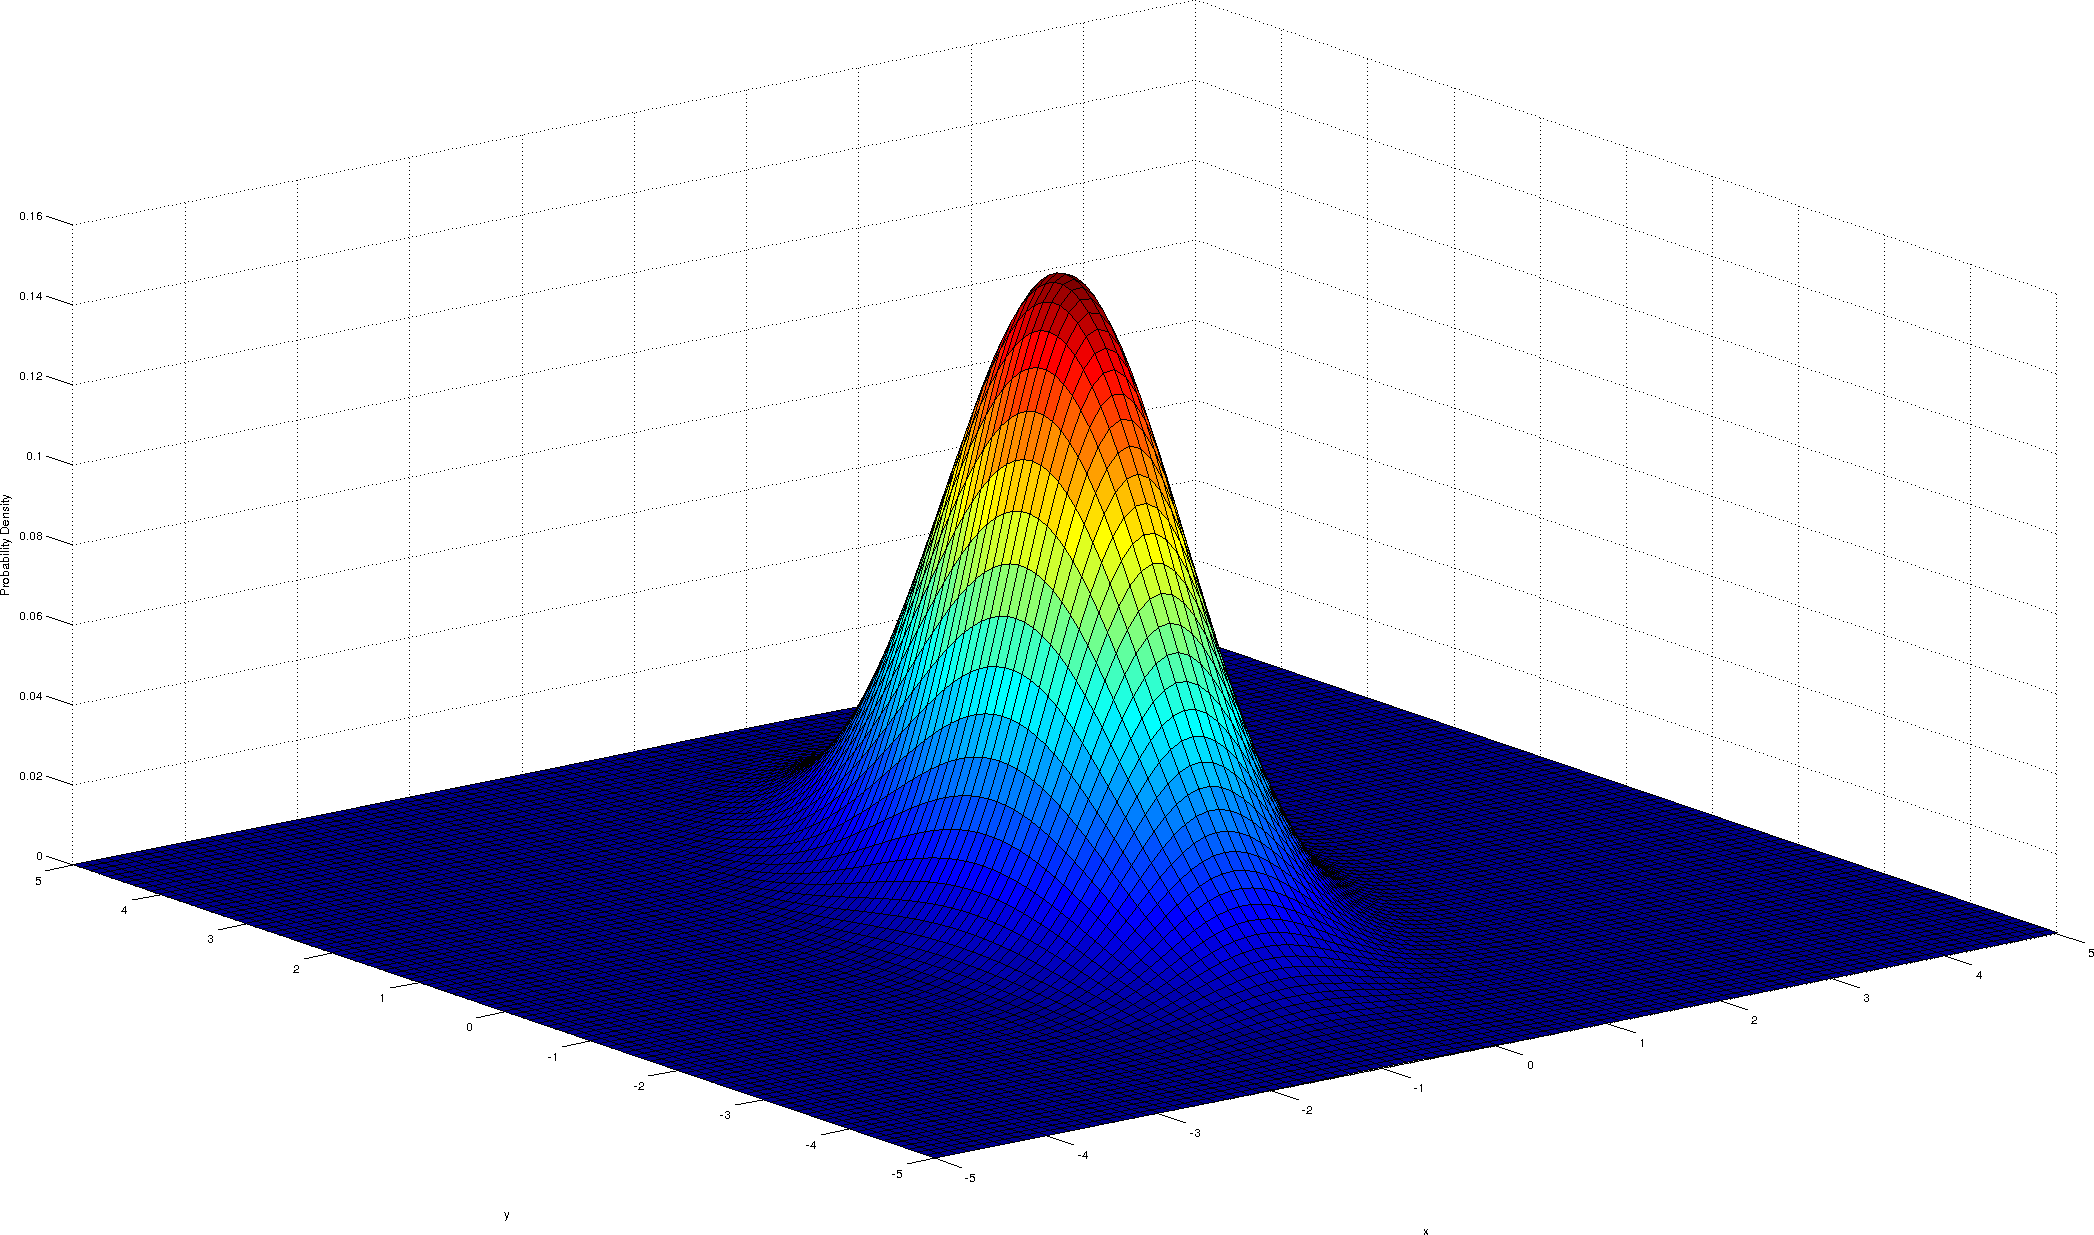
\includegraphics[width=\textwidth]{mvn_appendix_iso.png}
	\caption{caption goes here}
	\label{fig:some_nice_label_for_this_image}
\end{figure}



\begin{figure}[hptb]
        \centering
        \begin{subfigure}[b]{0.3\textwidth}
                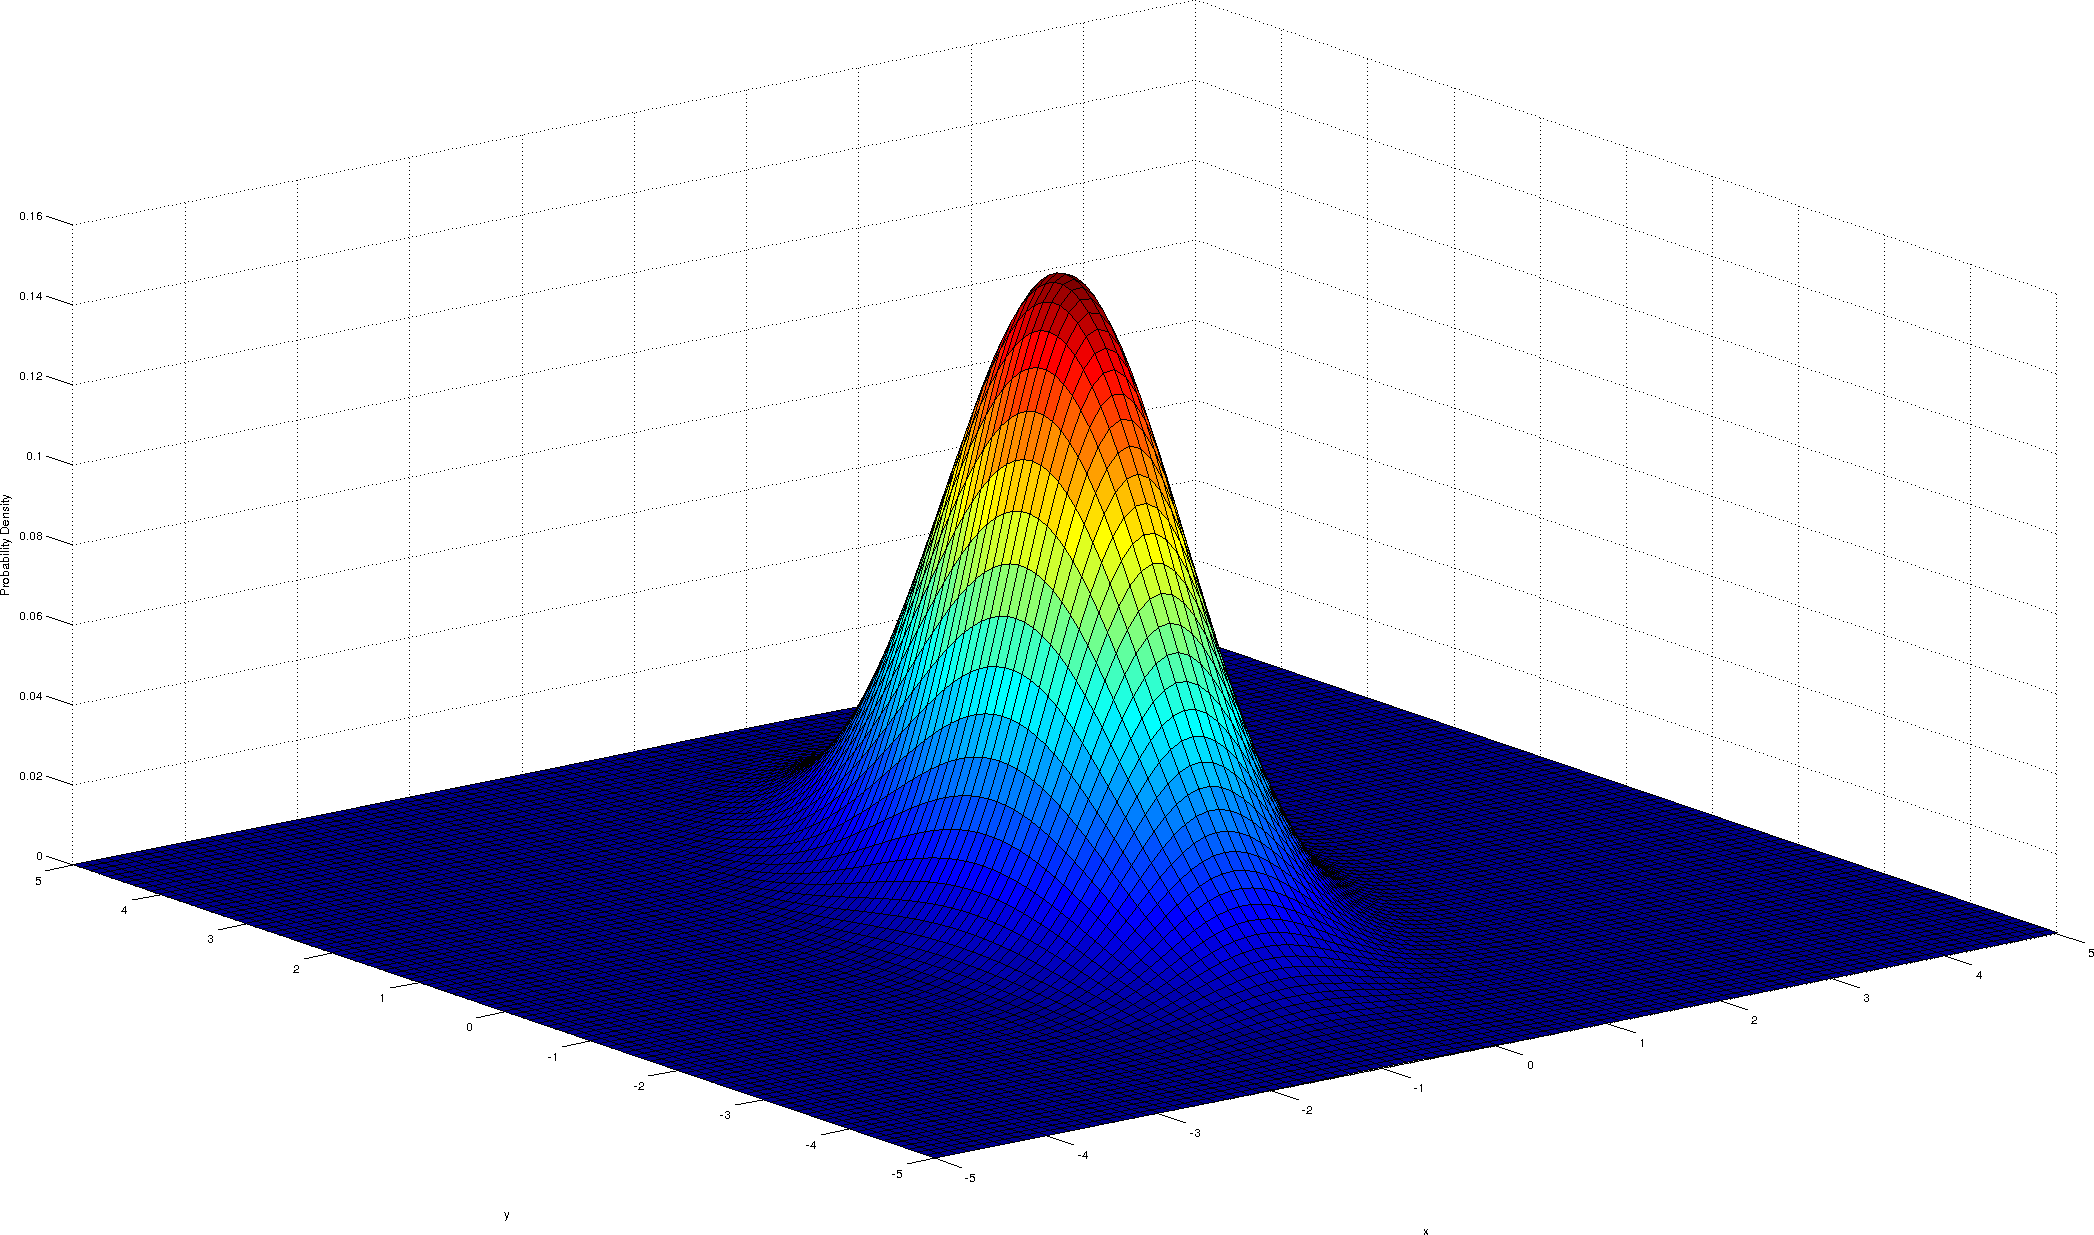
\includegraphics[width=\textwidth]{mvn_appendix_iso.png}
                \caption{caption}
                \label{fig:gull}
        \end{subfigure}%
        ~ %add desired spacing between images, e. g. ~, \quad, \qquad etc.
          %(or a blank line to force the subfigure onto a new line)
        \begin{subfigure}[b]{0.3\textwidth}
                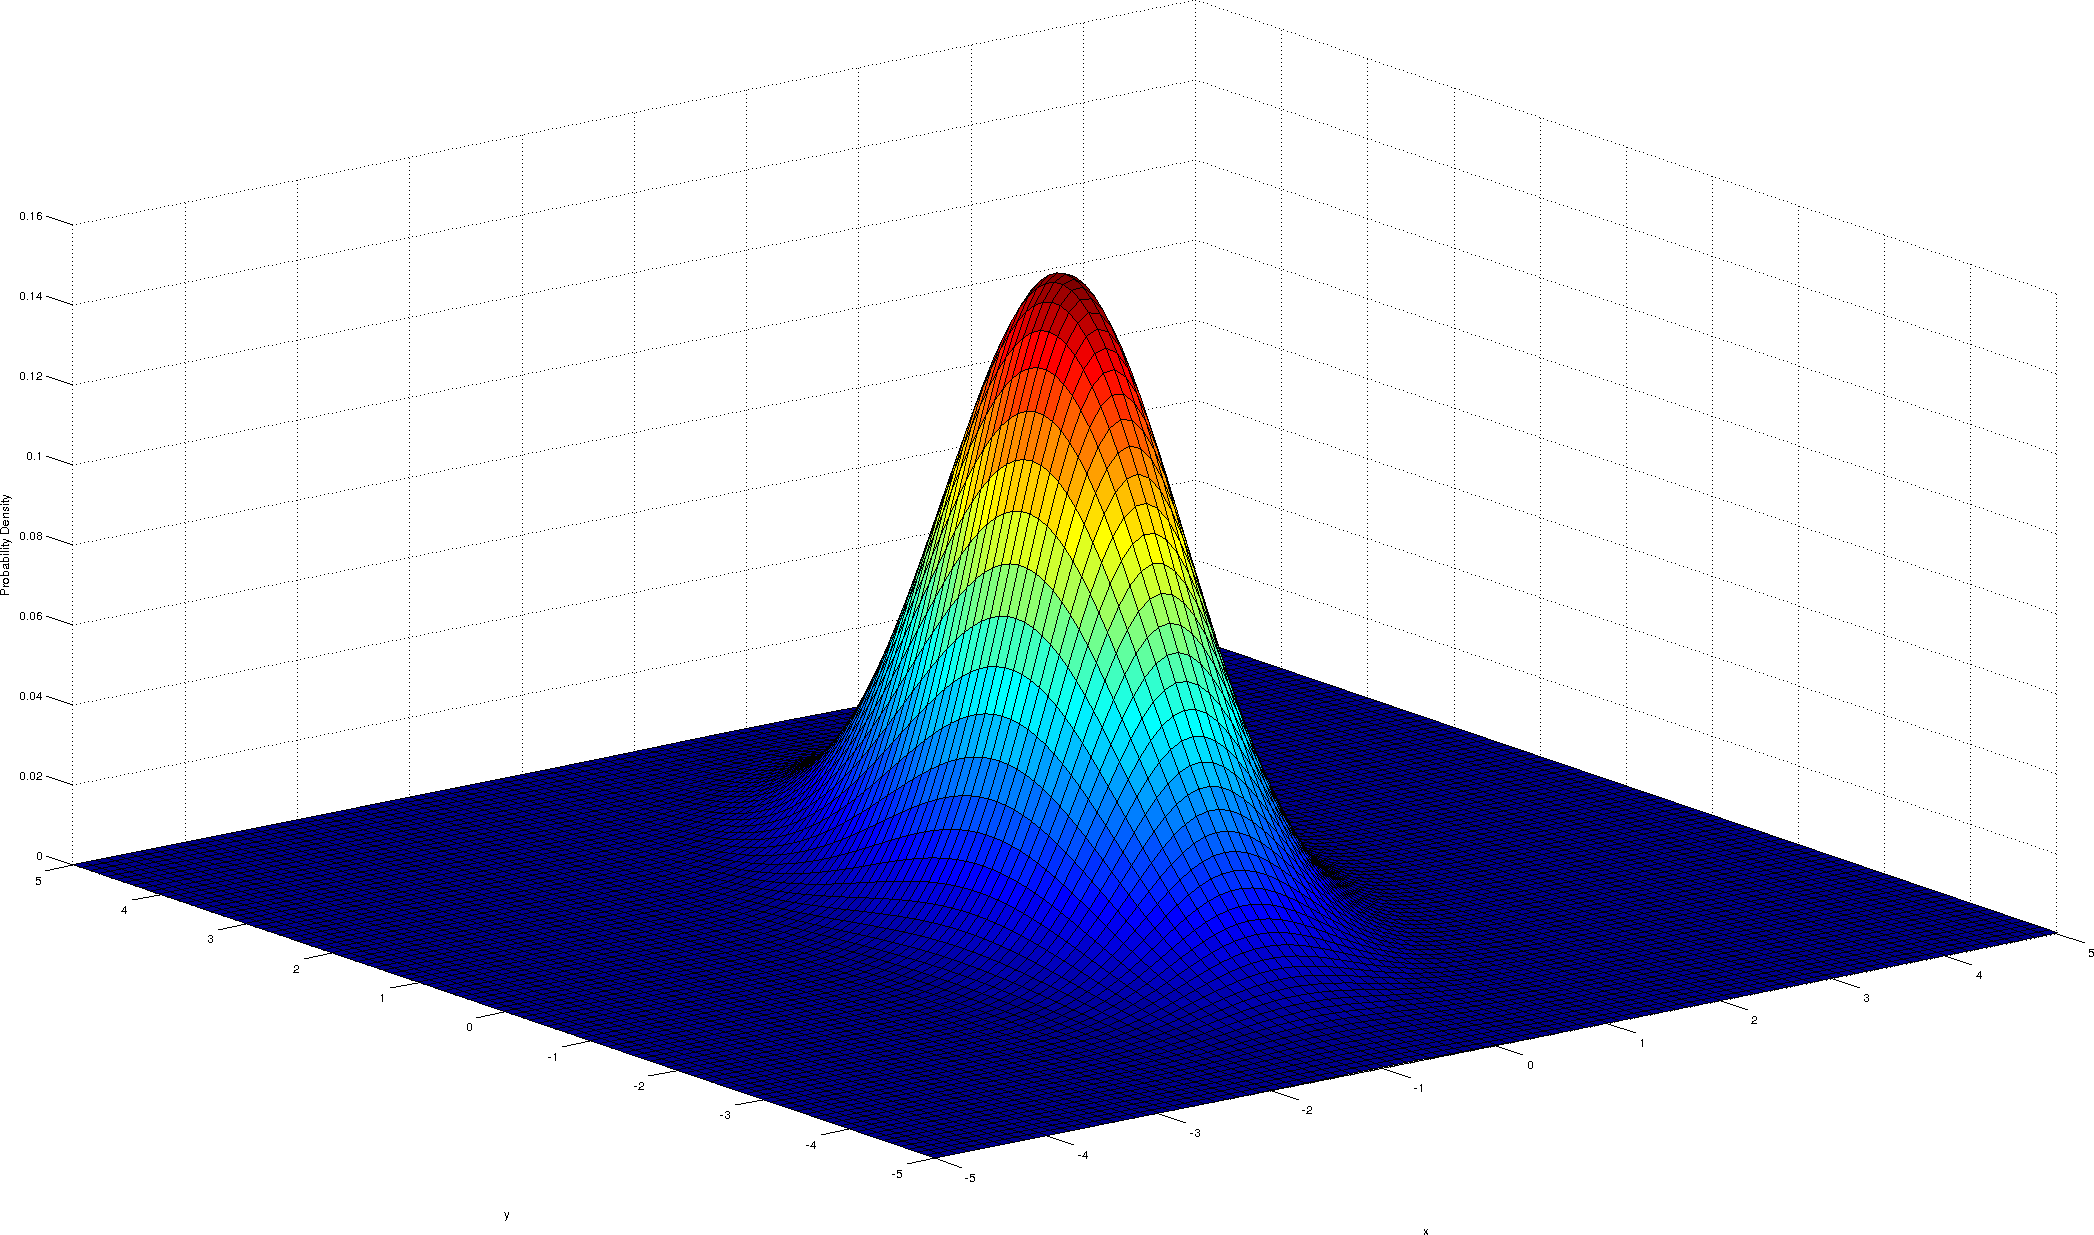
\includegraphics[width=\textwidth]{mvn_appendix_iso.png}
                \caption{caption}
                \label{fig:tiger}
        \end{subfigure}
        ~ %add desired spacing between images, e. g. ~, \quad, \qquad etc.
          %(or a blank line to force the subfigure onto a new line)
        \begin{subfigure}[b]{0.3\textwidth}
                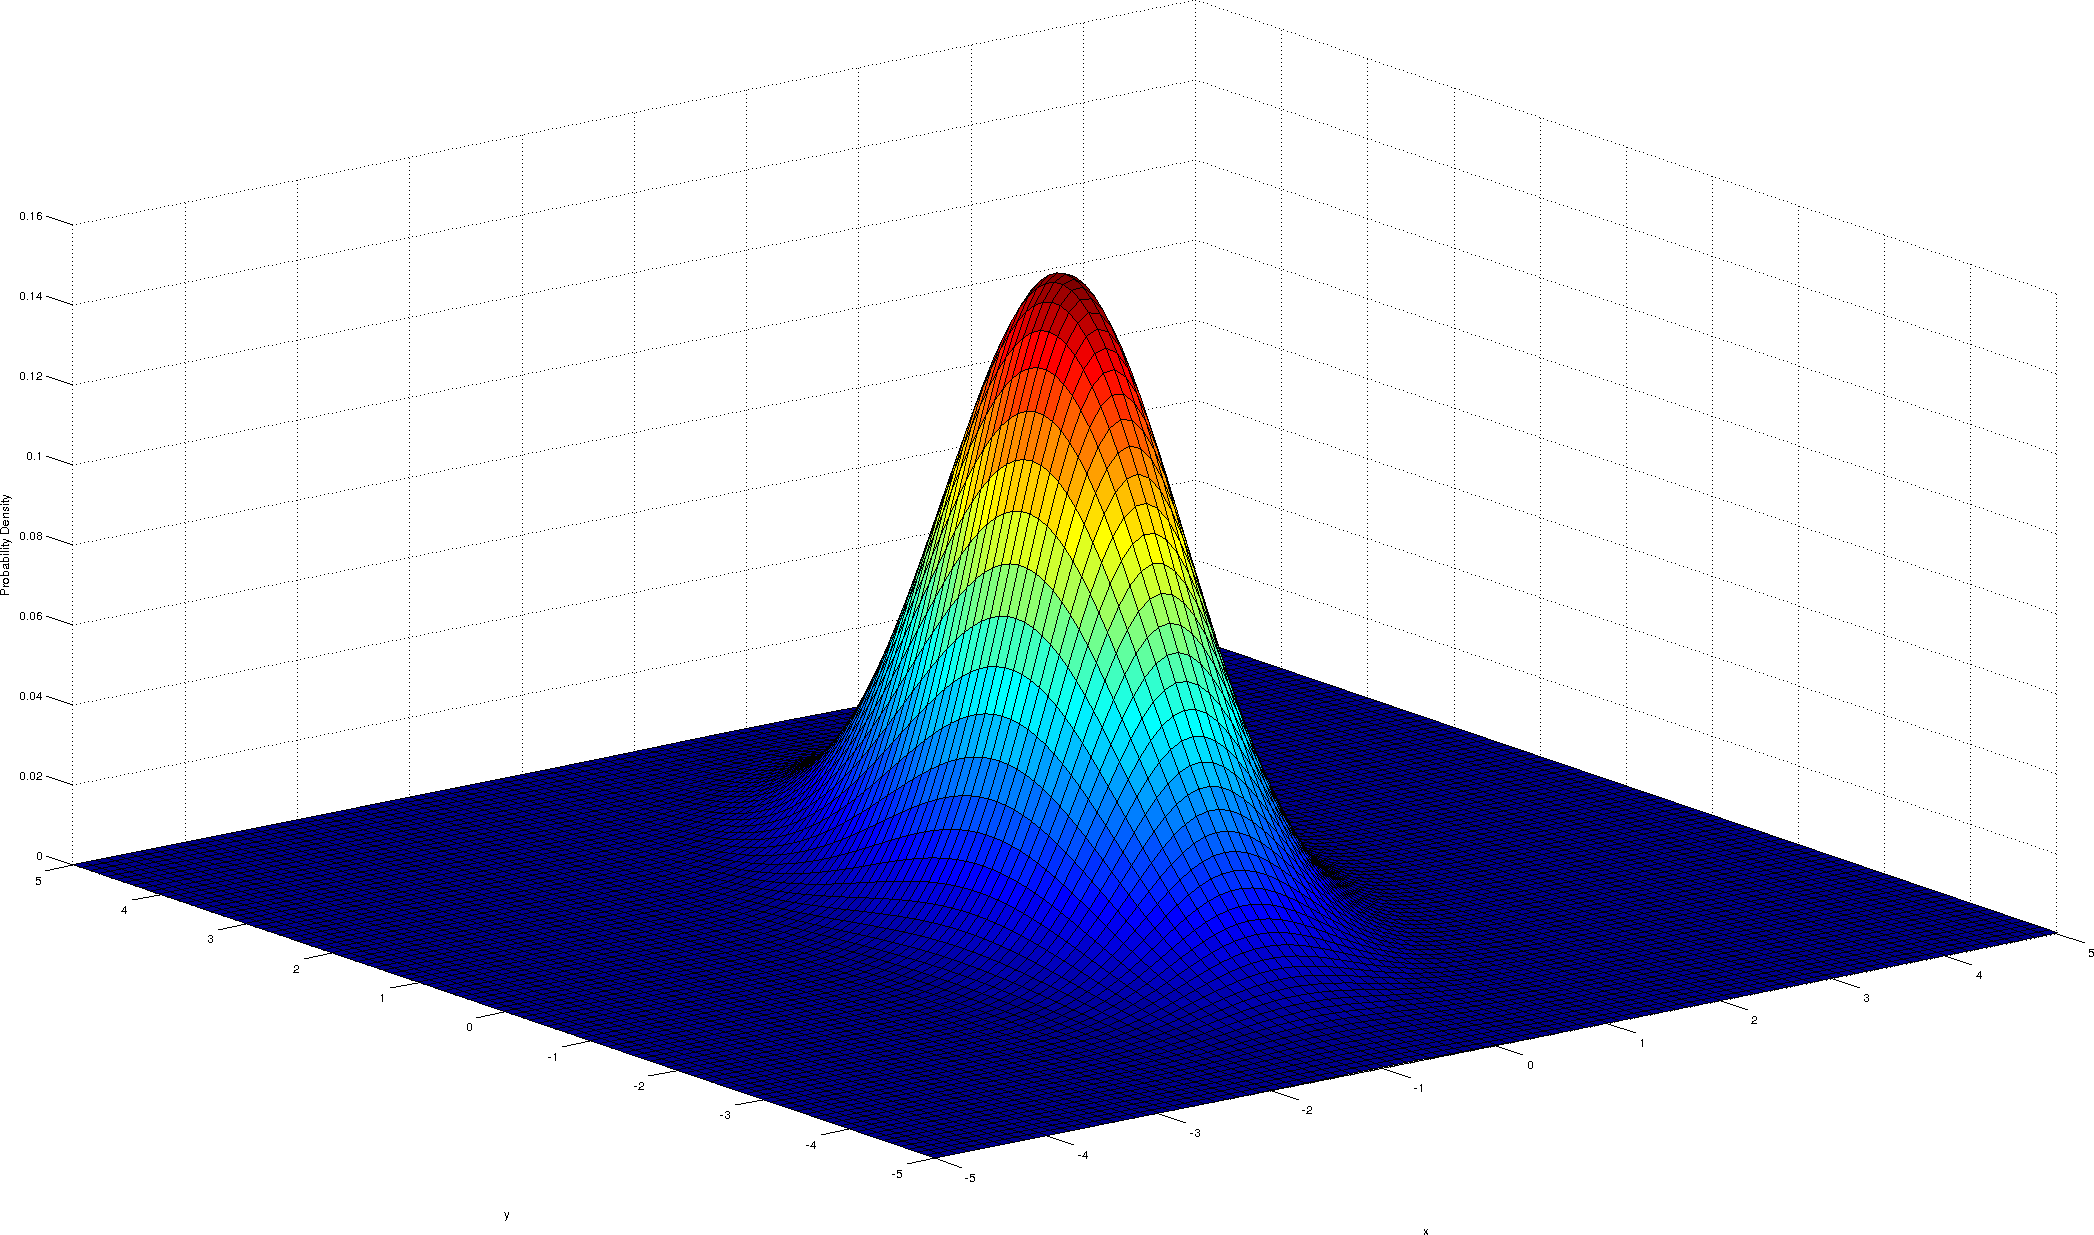
\includegraphics[width=\textwidth]{mvn_appendix_iso.png}
                \caption{caption}
                \label{fig:mouse}
        \end{subfigure}
        \caption{Pictures of something, horizontally}\label{fig:horizont}
\end{figure}



\begin{figure}[hptb]
	\centering
	\begin{subfigure}[t]{10cm}
		\centering
		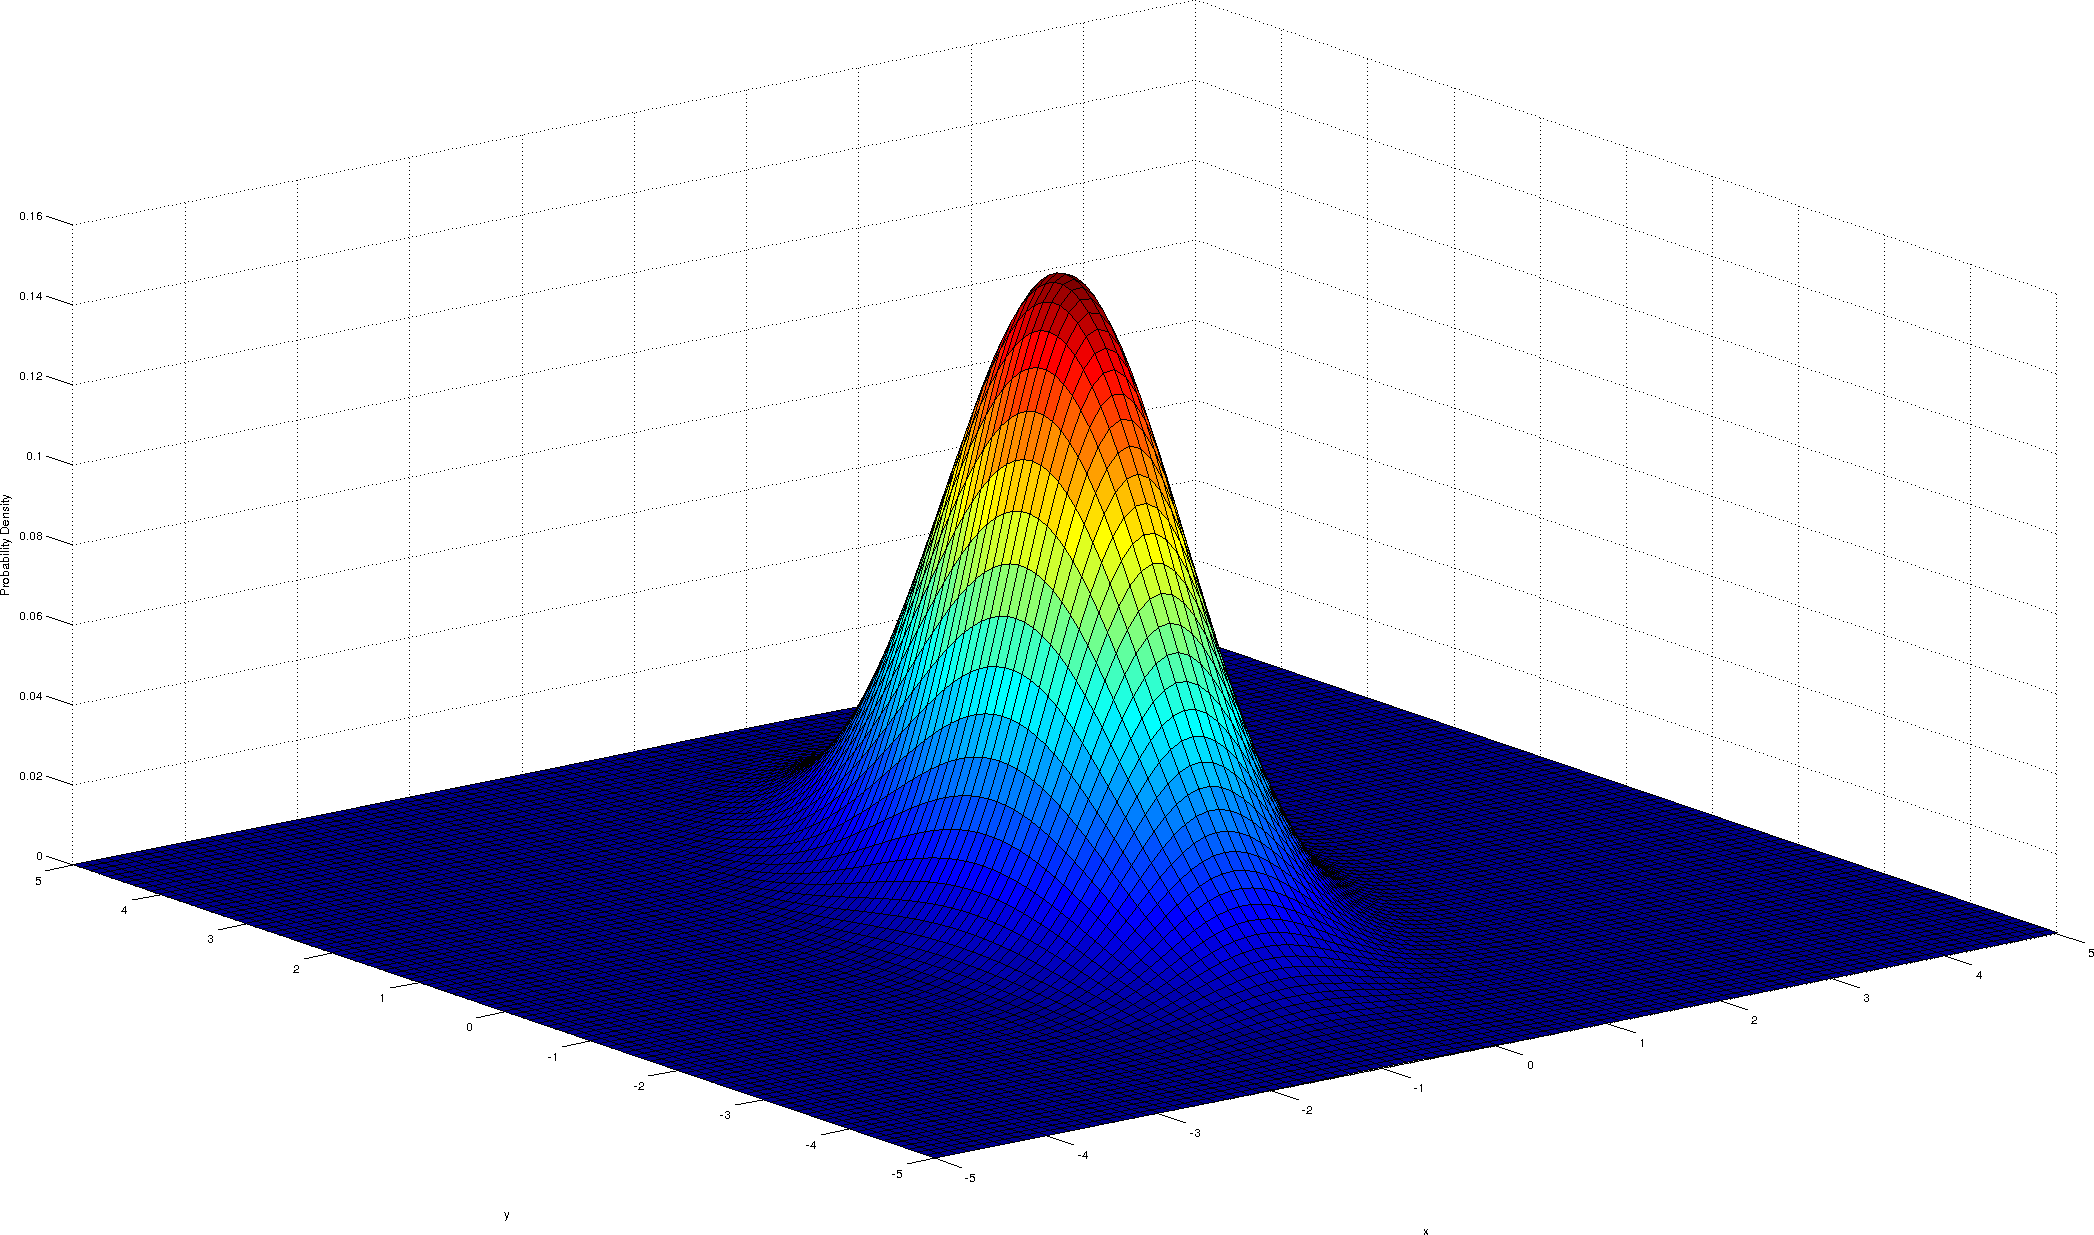
\includegraphics[width=10cm]{mvn_appendix_iso.png} 
		\caption{isometric perspective}
		\label{fig:app_mvn:iso}
	\end{subfigure}
	\begin{subfigure}[b]{\textwidth}
		\centering
		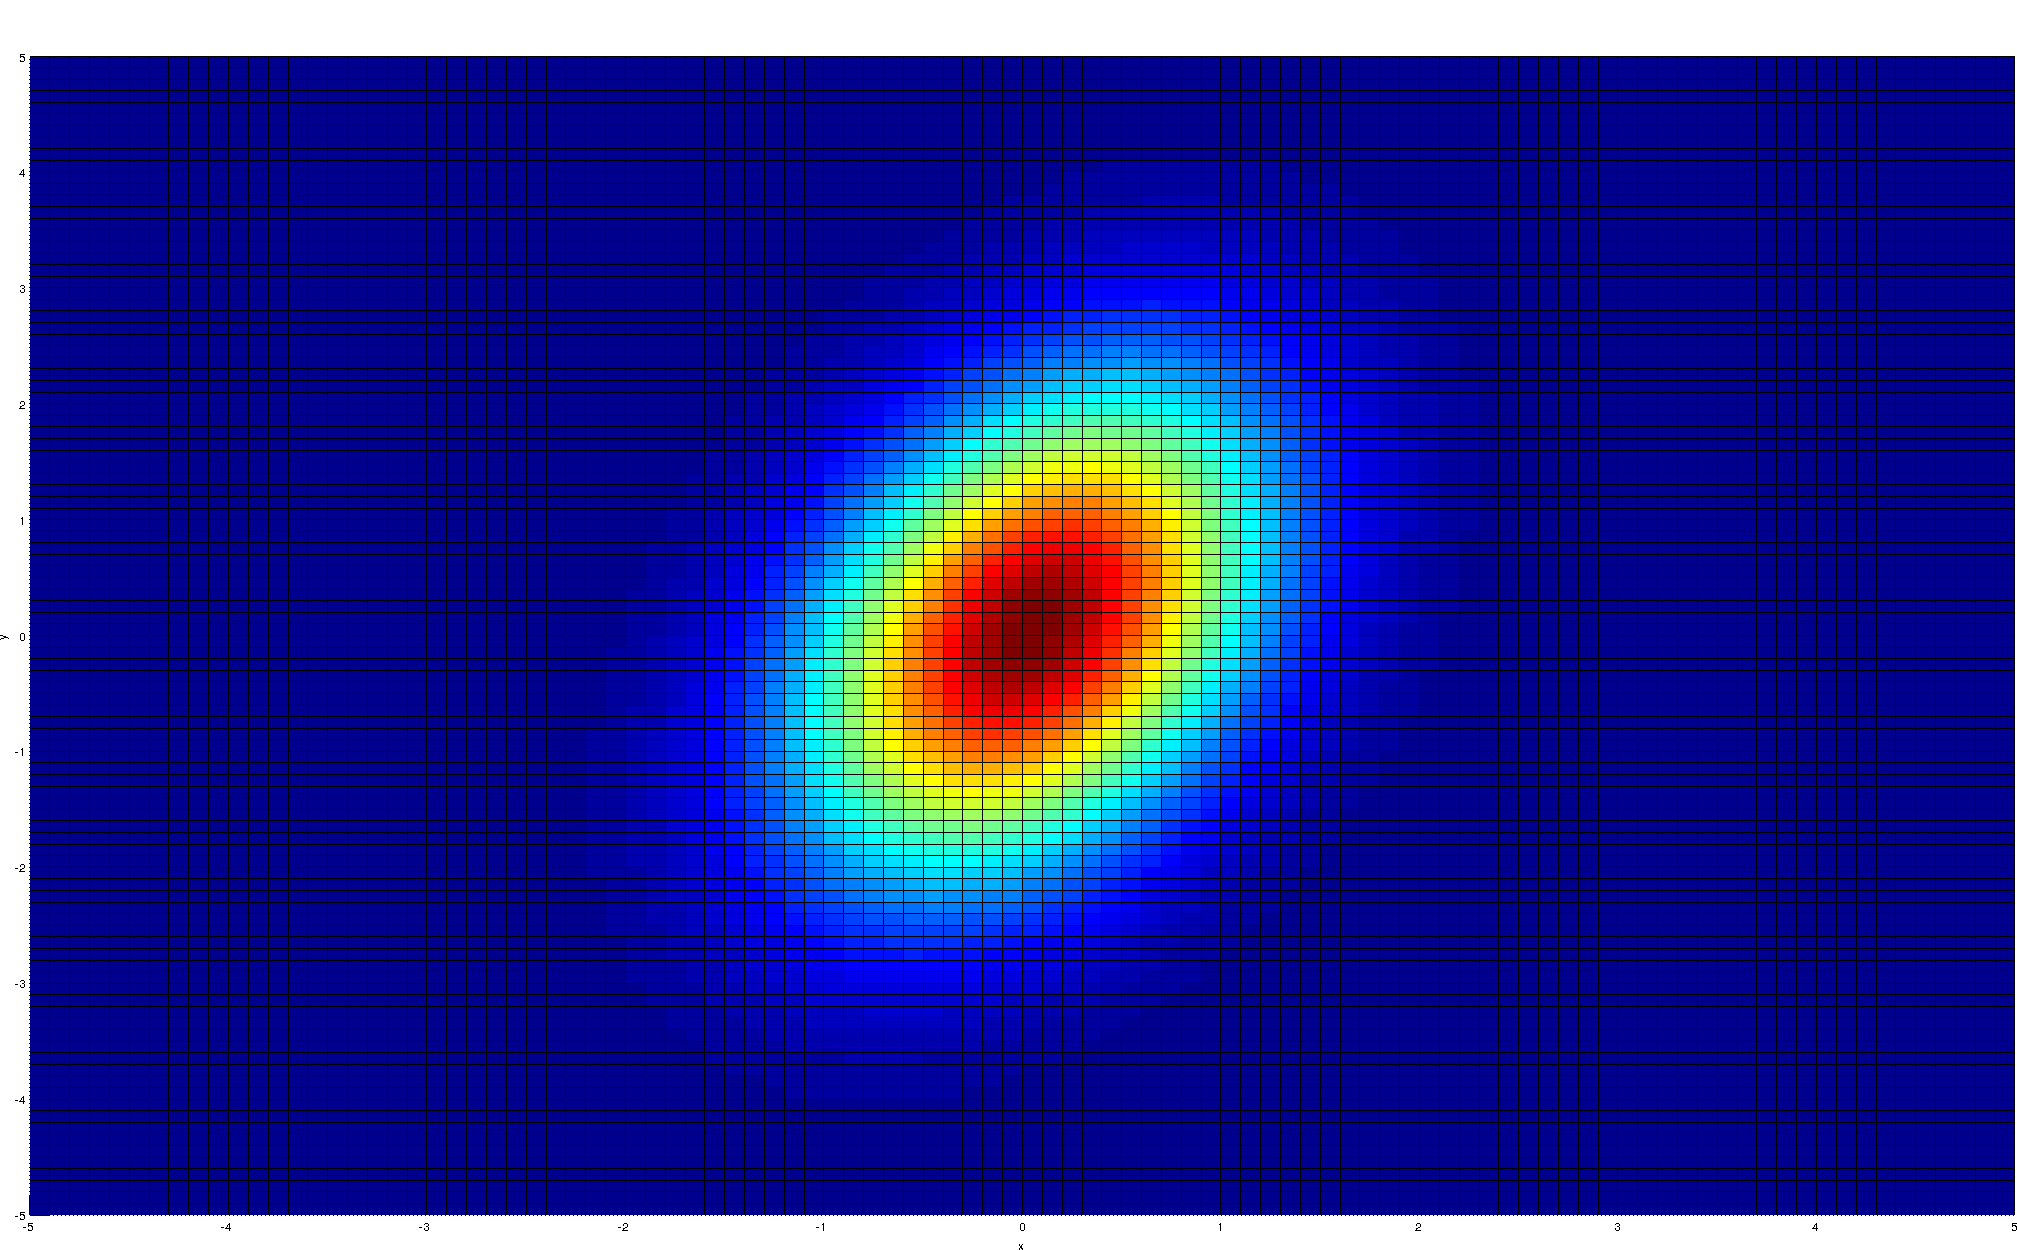
\includegraphics[width=10cm]{mvn_appendix_bird.png} 
		\caption{bird's eye view}
		\label{fig:app_mvn_bird}
	\end{subfigure}
	\caption[Multivariate Normal Distribution]{MVN with $\mu = \left[  
		\begin{array}{c} 
			0 \\ 
			0 
		\end{array} \right] $
		 and  $ \Sigma = \left[  
		\begin{array}{cc}
			0.6 & 0.4 \\ 
			0.4 & 2.0 \\
		\end{array} \right] $ }
	\label{fig:app_mvn}
\end{figure}







\newpage
\section{Math-Stuff}

Equations with explanations:
\begin{gather}
	p\left(x(k) \; \big| \; X^{k-1}, Z^{k-1}, U^k\right)
	\label{eq:bayes_1}
	\intertext{Where:}
	\begin{tabular}{>{$}r<{$}@{\ :\ }l}
		X^{k-1} := \{x(k-1), x(k-2), ..., x(0)\} & all previous states \\
		Z^{k-1} := \{z(k-1), z(k-2), ..., z(0)\} & all previous measurements \\
		U^k		:= \{u(k), u(k-1), ..., u(0)\} & all previous control inputs \\
	\end{tabular}\nonumber
\end{gather}

You can automatically refer to the beforehand stated equation~\ref{eq:bayes_1}. Pages with only math stuff sometimes looks strange. So make sure to add some nice text. 

\lipsum[0-1]


A list of equations aligned at the "=" symbol.
\begin{align}
	x(k+1|k) &= F(k) \cdot x(k|k) + G(k) \cdot u(k) 			\label{eq:kal_pred_x}	\\
	P(k+1|k) &= F(k) \cdot P(k|k) \cdot F(k)^T + Q(k) 			\label{eq:kal_pred_P}	\\
	\hat{z}(k+1|k) &= H(k+1) \cdot x(k+1|k) 					\label{eq:kal_pred_z}	\\
	S(k+1)   &= H(k+1) \cdot P(k+1|k) \cdot H(k+1)^T + R(k+1)	\label{eq:kal_pred_S}
\end{align}

References to Equation~\ref{eq:kal_pred_x} and  Equation~\ref{eq:kal_pred_z}

Write some matrices: $x = \begin{bmatrix}
x_{pos} \\
x_{vel} \\
y_{pos} \\
y_{vel}
\end{bmatrix}$ and $F = \begin{bmatrix}
1 & T & 0 & 0 \\
0 & 1 & 0 & 0 \\
0 & 0 & 1 & T \\
0 & 0 & 0 & 1
\end{bmatrix}$. 

\section{citing stuff}

You can cite stuff. For example an online resource \cite{adac_night}. Make sure to add a "laste visited" in JabRef. This has to appear in the bibliography. But you can also cite from a book, including the page number: \cite[p. 175]{mitchell1997}. And also inproceedings \cite{julier97} and articles \cite{Jin2003}. And technical manuals \cite{adma}.


\section{Tables}


\begin{table}[hbt]
	\begin{tabular}{p{4.0cm}C{3.6cm}C{4.0cm}}
		\toprule
		\textbf{Property}		&	\textbf{Stereo Camera}		&	\textbf{Multi-Mode Radar \newline (near / far)}	\\
		\midrule
		meas. principle	&	CMOS sensor			&	FMCW			\\
		cycle time		&	60ms				&	66ms			\\
		latency			&	42ms				&	198ms			\\
		\midrule
		frequency		&	16fps				&	76 - 77 Ghz		\\
		bandwidth		&	---					&	187 Mhz			\\
		\midrule
		opening angle	&	45°					&	60° / 18°			\\
		range			&	500m \newline (3D-vision: 50m)	&	~60m	/ 200m		\\
		\midrule
		angle accuracy ($3\sigma$)		&	---	&	~~$\pm$ 1° / $\pm$ 0.1°		\\
		distance accuracy ($3\sigma$)	&	---	&	$\pm$ 0.25m		\\
		velocity accuracy ($3\sigma$)	&	---	&	$\pm 0.278 \tfrac{m}{s}$ / $\pm 0.139 \tfrac{m}{s}$	\\
		\bottomrule
	\end{tabular}
	\caption{Overview of the properties of several sensors}
	\label{tab:sensor_properties}
\end{table}


\begin{table}[H]
	\centering
	\begin{tabular}{r|ccc|ccc}
	\toprule
       &  \multicolumn{3}{c|}{\textbf{full}}      & \multicolumn{3}{c}{\textbf{diag}}  \\
           &    RMSE &  PVol & NEES  & RMSE  & PVol & NEES        \\
    \midrule
    sensor-1    &    1.63   &  0.69 &  3.79   &    1.63 &   1.27 &     3.90     \\
    sensor-2    &    1.14   &  0.85 &  4.23   &    1.14 &   1.56 &     4.28     \\
    CMF         &    0.84   &  0.15 &  3.82   &    0.84 &   0.15 &     3.82     \\
  \midrule
    Naive       &    1.37   &  1.80 &  2.24   &    1.37 &   2.70 &     2.43     \\
    CI-trace    &    1.26   &  0.62 &  2.68   &    1.27 &   1.12 &     2.77     \\
    CI-det      &    1.37   &  0.61 &  3.31   &    1.34 &   1.11 &     3.16     \\
    Bar-Shalom-0.0      &    1.25   &  0.16 &  4.90   &    1.25 &   0.29 &     5.12     \\
    Bar-Shalom-0.4      &    1.21   &  0.25 &  4.04   &    1.22 &   0.46 &     4.09     \\
    Bar-Shalom-0.7      &    1.19   &  0.21 &  5.86   &    1.19 &   0.41 &     5.27     \\
    \midrule
    IMF         &    1.05   &  0.22 &  3.85   &    0.93 &   0.14 &     5.34     \\
    KF-T2T      &    1.80   & 12.17 & 7.15   &    1.64  &  11.76 &     5.32     \\
    IMF-sub     &    1.18   &  0.12 & 12.75   &    1.18 &   0.21 &    13.35     \\
	\bottomrule
	\end{tabular}
	\caption{some random numbers}
	\label{tab:res_prob1_vel_rmse}
\end{table}




\begin{table}[hbt]
\centering
\begin{small}
	\begin{tabular}{C{5.8cm}C{5.8cm}}
	\toprule
	\textbf{trainings set} & \textbf{validation set} \\
	\midrule
		$P_{C} = \begin{bmatrix}
			 0.307	&	 0.574	&	0	&	0	\\
			 0.574	&	 4.926	&	0	&	0	\\
			0	&	0	&	 0.052	&	 0.080	\\
			0	&	0	&	 0.080	&	 0.384	
		\end{bmatrix}$
		\newline
		$P_{R} = \begin{bmatrix}
			 0.066	&	 0.168	&	0	&	0	\\
			 0.168	&	 3.025	&	0	&	0	\\
			0	&	0	&	 0.360	&	 0.298	\\
			0	&	0	&	 0.298	&	 0.725	
		\end{bmatrix}$
		&
		$P_{C} = \begin{bmatrix}
			 0.301	&	 0.536	&	0	&	0	\\
			 0.536	&	 4.886	&	0	&	0	\\
			0	&	0	&	 0.054	&	 0.087	\\
			0	&	0	&	 0.087	&	 0.403	
		\end{bmatrix}$
		\newline
		$P_{R} = \begin{bmatrix}
			 0.071	&	 0.182	&	0	&	0	\\
			 0.182	&	 3.151	&	0	&	0	\\
			0	&	0	&	 0.356	&	 0.298	\\
			0	&	0	&	 0.298	&	 0.699	
		\end{bmatrix}$
\\
	\bottomrule
	\end{tabular}
\caption{covariances}
\label{tab:sol_stistical_emp_P_sim}
\end{small}
\end{table}




\section{Pseudo Algorithm}

For computer scientists: Write some pseudo code:

\begin{algorithm} 
	\begin{algorithmic}
		\Require $F$, $R$, $H$, $dt$ of the sensor
		\While {optimizing}
			\State select $q$
			\State calculate $P$ using alpha-beta equation
			\State calculate NEES
			\If {current NEES better than best NEES}
				\State $P_{ab} \gets P$
				\State best NEES $\gets$ current NEES
			\EndIf
		\EndWhile
		\State \Return {$P_{ab}$}
	\end{algorithmic}
	\caption{Pseudocode of the optimization process for $P_{ab}$}
	\label{algo:opti}
\end{algorithm} 

And explain it afterwards. 

\lipsum[1-2]



\section{Rotated Tables}
\vfill
\begin{center}
   \hvFloat[%
    nonFloat=true,%
    capPos=r,%
    capAngle=90,%
    capWidth=h,	% of \columnwidth
    capVPos=c,%
    objectAngle=90,%
]{table}{%
	% less padding around math environments
	\setlength{\abovedisplayskip}{50pt}	%
	\setlength{\belowdisplayskip}{50pt}	%
    \begin{tabular}{lL{2.5cm}L{10.5cm}c}	%
	\toprule
	 		& \textbf{needed data} & \textbf{equations} & \textbf{optimal}   \\ 
	\midrule
	CI 	
		&
		$ P_i$, $P_j $			\newline 
		$ \omega \in (0, 1) $
		&
		$ P^{-1} = \omega P_i^{-1} + (1 - \omega)P_j^{-1} $	\newline \vspace{5pt}
		$ \hat{x} = P \cdot [ \; \omega P_i^{-1}\hat{x}_i + (1 - \omega) P_j^{-1}\hat{x}_j \; ]$
		&	no		\\ 
	\midrule 
	BarS. 1				
		&	
		$P_i$ , $P_j$	\newline
		&	
		$ \hat{x} = P_j(P_i+P_j)^{-1}\hat{x}_i + P_i(P_i + P_j)^{-1}\hat{x}_j  $	\newline \vspace{5pt}
		$ P = P_1(P_i + P_j)^{-1}P_j $	
		&	no		\\ 
	\midrule 
	BarS. 2	
		&	
		$P_i$, $P_j$, $P_{ij}$, \newline
		$P_{ji}$, $K_i$, $K_j$, \newline
		$H_i$, $H_j$, 			
		$F$, $Q$
		&	
		$ \hat{x} = \hat{x}_i + [P_i - P_{ij}][P_i + P_j - P_{ij} - P_{ji}]^{-1}[\hat{x}_j - \hat{x}_i] $	 \newline \vspace{5pt}
		$ P = P_i - [P_i - P_{ij}][P_i + P_j - P_{ij} - P_{ji}]^{-1}[P_i - P_{ji}]$	\newline \vspace{5pt}
		$ P_{ij} \approx 0.4 \cdot \sqrt{P_i \circ P_j} $
		&	yes		\\ 
	\midrule
	IMF 			
		&
			$\hat{x}_i(k|k-1)$	\newline
			$\hat{x}_i(k|k)$		\newline
			$P_i(k|k-1)$			\newline
			$P_i(k|k)$			\newline
			$ \hat{x}(k|k-1) $	\newline
			$ P(k|k-1)$			\newline
			$F$, $Q$
		&	
		\newline 
		$ P(k|k)^{-1} = \sum_{i=1}^2 \left[ P_i(k|k)^{-1}  - P_i(k|k-1)^{-1} \right]  + P(k|k-1)^{-1} $	\newline \vspace{5pt}
		$ \hat{x}(k|k) = P(k|k) \cdot \{ \; P(k|k-1)^{-1} \cdot \hat{x}(k|k-1)  $	\newline \vspace{5pt}
		$	 \qquad	\qquad		 + \sum_{i=1}^2 \left[ P_i(k|k)^{-1} \hat{x}_i(k|k) - P_i(k|k-1)^{-1} \hat{x}_i(k|k-1) \right] \; \}	$
		&	yes		\\
	\bottomrule
    \end{tabular}
}[hpbt]{Summary of the used track-to-track fusion algorithms}{tab:t2t_summarytable}
\end{center}
\vfill\clearpage

